W pewnym momencie projektu zapad�a decyzja o zmianie platformy na kt�rej b�dziemy budowa� quadrocopter. W tym celu postanowiono o zaprojektowaniu i wykonaniu nowych \textbf{Center Plate'�w} dla platformy. Center Plate s� to dwie p�ytki, znajduj�ce si� na �rodku ramy, do kt�rych mocowane s� ramiona i podzespo�y quadrocoptera takie jak:
\begin{itemize}
\item sterownik i odbiorniki
\item GPS
\item bateria
\item komputer pok�adowy (sterownik nadrz�dny)
\item modu� FPV
\item podwozie
\item oraz pozosta�e elementy wyposa�enia drona 
\end{itemize}
Nowozaprojektowane p�ytki musia�y odpowiada� pewnym za�o�eniom. Otwory do monta�u ramion i podwozia musia�y by� �atwo dost�pne. Dodatkowo nale�a�o umie�ci� otwory monta�owe dla sterownika nadrz�dnego, odbiornik�w, baterii itd. \\ 
Projekt powsta� w programie \textit{AutoDesk AutoCAD 2014}. Wykonany zosta� rysunek wykonawczy p�ytki g�rnej oraz dolnej \ref{fig:center_top}. Dodatkowo zadbano o zastosowanie odpowiednich wyci�� dla uzyskania ni�szej masy w�asnej. 
\begin{figure}[htp]
\centering
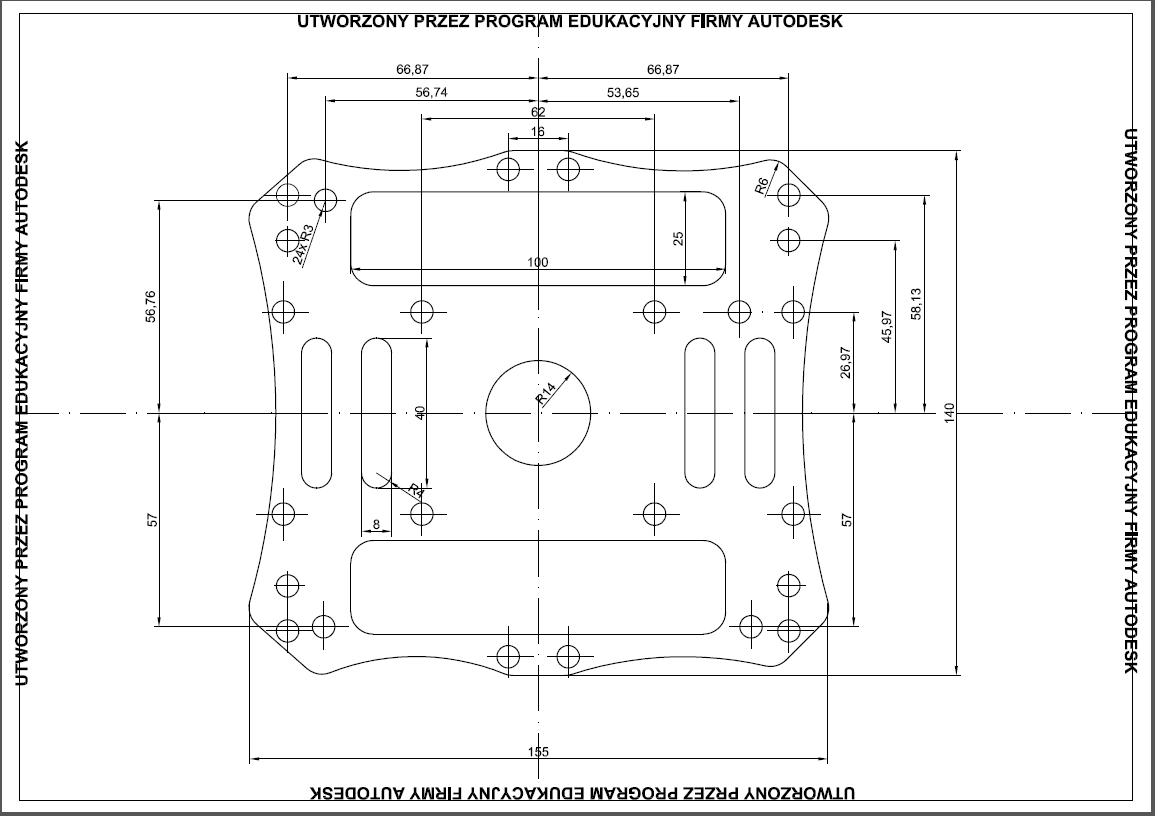
\includegraphics[width=\textwidth]{./grafika/center_top.png}
\caption{Projekt p�ytki Center Plate wykonany w programie AutoCAD 2014}
\label{fig:center_top}
\end{figure}

Pomimo, �e Center Plate zosta� wykonany, ostatecznie postanowiono wykorzysta� gotowy produkt \textbf{DJI F450 KIT} zakupiony w sklepie \url {www.abc-rc.pl/DJI-F450-DJI0233}. 
